%!TEX root = Zusammenfassung.tex

\section{Mathematische Grundlagen}
% ---------------------------------------------------------------------------------------------------------------------
\subsection{Ordnungen}
\begin{enumerate}
	\item (partielle) Ordnung: reflexiv, transitiv, antisymmetrisch
	\item minimale, maximale Elemente: fehlende Existenz von kleineren, größeren Elementen
	% komponentenweise Ordnung
	\item größtes, kleinstes Element: alle anderen sind kleiner, größer
	% Verband der Teilmengenrelation
	\item totale Ordnung: beliebige zwei Elemente vergleichbar
	\item Kette, Antikette: Menge von nur (un-)vergleichbaren Elementen, genauer:
		$A \text{ Antikette } \Leftrightarrow (\forall x,y \, :\, x,y\in A \land x\not= y : \neg ((x\leq y) \lor  (y\leq x)))$
	\item maximale (Anti-) Kette: es gibt keine echte Obermenge, die eine \hbox{(Anti-)} Kette ist.
		Maximale Antiketten sind als Mengen partiell geordnet
	\item Theorem 1.1 in \cite{Ban93}.
	\item lexikographische, komponentenweise Ordnung: sollten bekannt sein.
\end{enumerate}

% ---------------------------------------------------------------------------------------------------------------------
\subsection{Graphen}

\begin{enumerate}
	\item (un)gerichtete Graphen: Knoten, Bögen/Kanten (mit/ohne Richtung) (Anm: wir verwenden ``Kanten'' auch im gerichteten)
	\item Wege, Pfade: klar; Pfad beachtet die Richtung
	\item Zyklen, Schleifen: Weg, Pfad mit Anfang = Ende
	\item schwach zusammenhängend: ungeachtet der Richtung
	\item stark zusammenhängend: mit Beachtung der Richtung von jedem zu jedem
	\item $n$-fach zusammenhängend: nach dem Löschen von $n\!-\!1$ beliebigen Kanten immer noch zusammenhängend
	\item schwache, starke Zusammenhangskomponenten: Teilgraphen, die schwach, stark zusammenhängend sind
	\item azyklische Kondensation: pro starke Zusammenhangskomponente ein Knoten; die ``schwachen Kanten'' übernehmen
\end{enumerate}

\textbf{Beispielgraph:}

\begin{center}
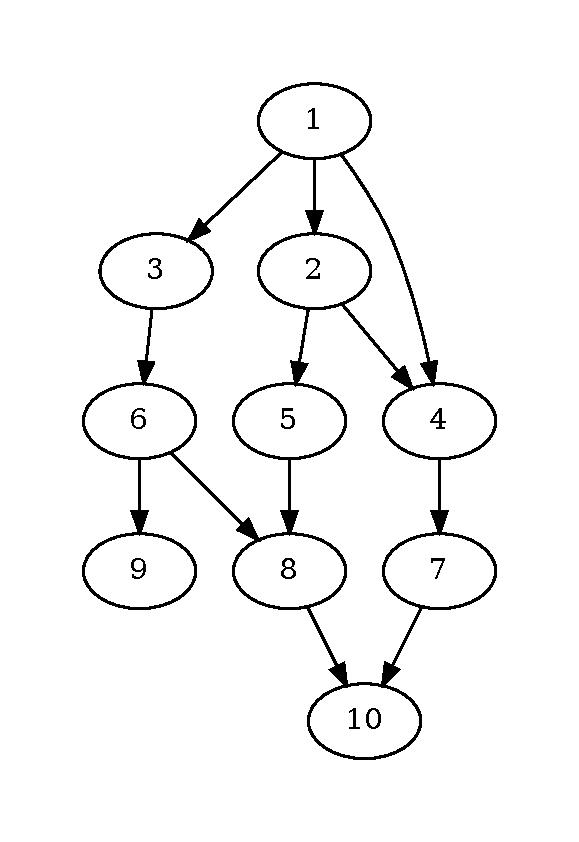
\includegraphics[scale=0.7]{images/BeispielgraphGraphentheorie.pdf}
\end{center}

\subsubsection{Bestimmung maximaler Ketten}
Von der $1$ an beginnend den Baum aufbauen, Knoten streichen wenn sie durch einen längeren
Pfad erreicht werden können. Tritt ein Knoten mehrfach mit gleicher Distanz zum Anfangsknoten
auf, bleiben beide Ketten bestehen. Sind alle Kanten ausgeschöpft, mit einem anderen Knoten von
vorne beginnen, der noch in keinem Baum aufgetaucht ist (Im Beispiel nicht der Fall).

Hier:
\[1 \rightarrow 3 \rightarrow 6 \rightarrow 9\]
\[1 \rightarrow 3 \rightarrow 6 \rightarrow 8 \rightarrow 10\]
\[1 \rightarrow 2 \rightarrow 5 \rightarrow 8 \rightarrow 10\]
\[1 \rightarrow 2 \rightarrow 4 \rightarrow 7 \rightarrow 10\]

\subsubsection{Bestimmung maximaler Antiketten}
Zunächst die transitive Hülle der Relation bestimmen. Das geschieht im Beispiel idealerweise
bei der 10 beginnend, da Kanten nur von kleineren zu größeren Zahlen existieren. Daraus können
die Antiketten der Länge 2 bestimmt werden. Diese lassen sich immer dann zu längeren Antiketten
verbinden, wenn $\{a,b\}, \{a,c\}, \{b, c\}$ Antiketten sind: Sie bilden zusammen $\{a,b,c\}$.
\textit{Maximale Antiketten} sind die mit der Länge $N$, wenn die längste Antikette $N$
Elemente hat.

Hier:
\[\{1\}, \{2,3\}, \{2,6\}, \{2,9\}, \{3, 4,5\}, \{3, 5, 7\}, \{4, 5, 6\}, \{4,5,9\}, \{4,8,9\},
\{5,6,7\},\{5,7,9\}, \{7,8,9\}, \{9,10\}\]

\subsubsection{Stark und schwach zusammenhängend}
\begin{itemize}
    \item Schwach zusammenhängend: Graph zerfällt nicht in unzusammenhängende Teilgraphen.
    \item Stark zusammenhängend: Jeder Knoten im Graph ist von jedem anderen aus erreichbar.
    \item $n$-fach zusammenhängend: nach dem Löschen von $n−1$ beliebigen Kanten immer noch zusammenhängend
    \item schwache, starke Zusammenhangskomponenten: Teilgraphen, die schwach, stark zusammenhängend sind
    \item azyklische Kondensation: pro starke Zusammenhangskomponente ein Knoten; die “schwachen Kanten” übernehmen
\end{itemize}

% ---------------------------------------------------------------------------------------------------------------------
\subsection{Matrixalgebra}
\textit{Siehe dumb.pdf Kapitel 3}

% ---------------------------------------------------------------------------------------------------------------------
\subsection{Fourier-Motzkin}